%%%%%%%%%%%%%%%%%%%%%%
%
%   Work related to the verification of the datasets
%
%%%%%%%%%%%%%%%%%%%%%%

\section{Slices of Datacubes}

\section{Power spectra from Theory}

\TODO{Provide some camb and class power spectra here. }

\section{Powerspectra from Simulations}
\begin{figure}
    \centering
    % 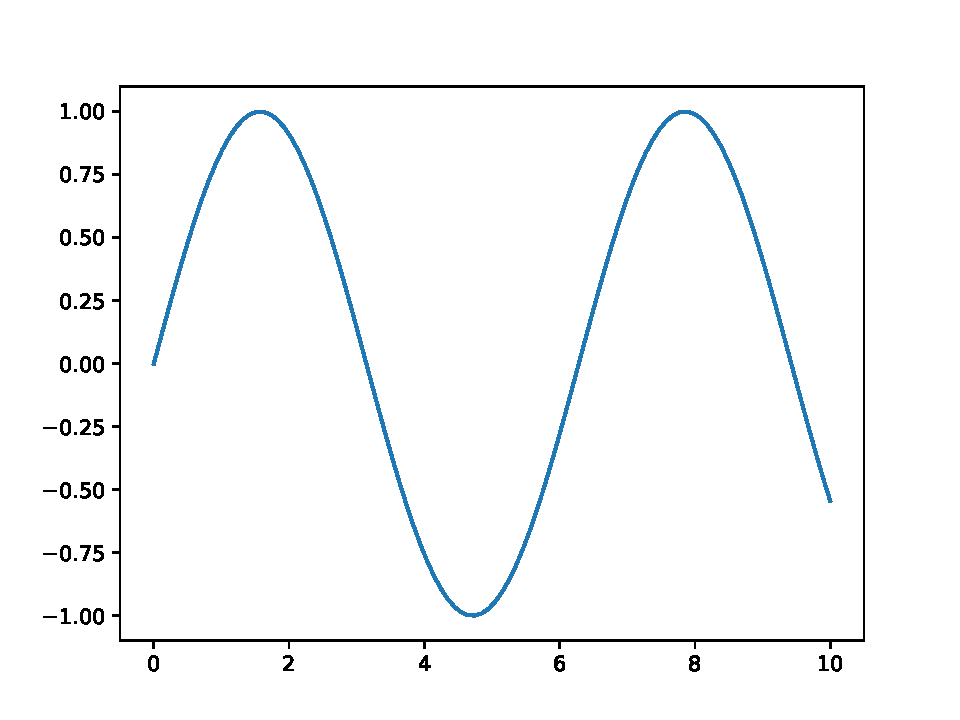
\includegraphics[width=\linewidth]{main/test.pdf}
    \includeimage[width=\linewidth]{nine_matter_power_spectra}
  \end{figure}

  \begin{figure}
    \centering
    % 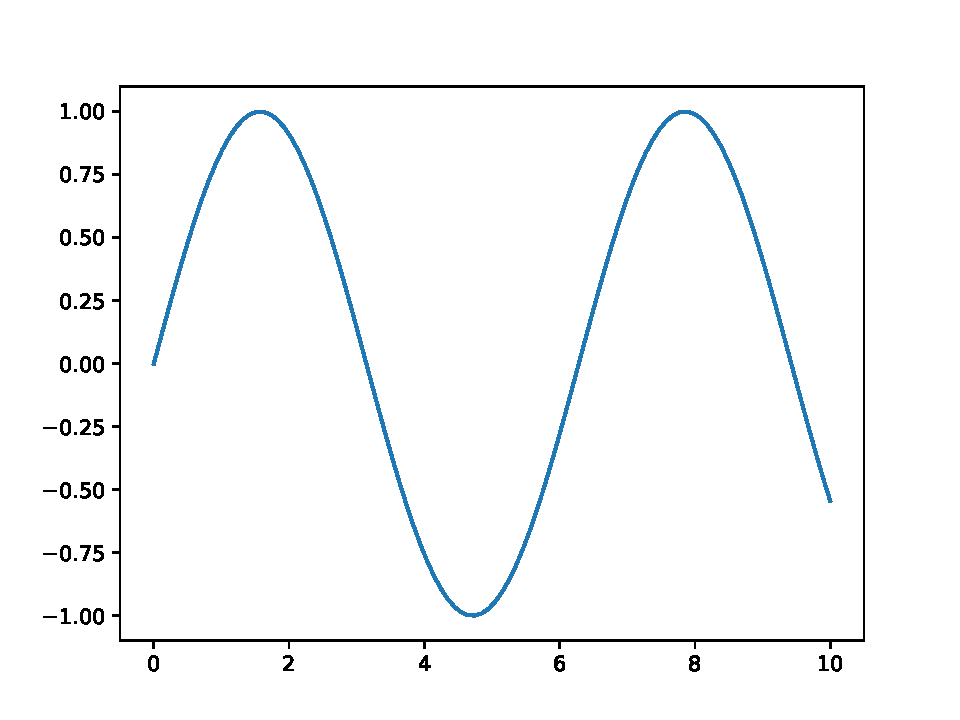
\includegraphics[width=\linewidth]{main/test.pdf}
    \includeimage[width=\linewidth]{average_matter_power_spectrum}
  \end{figure}

\section{Powerspectra from Datacubes}